\section{PG-GAT --- Pose Grouping Graph Attention Network}
\label{sec_meth_pggat}

This section describes the methodological centrepiece of the work:
PG-GAT, a skeleton-aware modification of the baseline GATv2 embedding network of Section~\ref{sec_meth_baseline}.
Three modifications to the attention mechanism are introduced,
each motivated by a specific failure mode of the baseline and each independently configurable for ablation,
and a two-stage training schedule (synthetic pre-training followed by COCO fine-tuning)
that is itself defended by a Bayesian sweep over fine-tune hyperparameters.
Every PG-GAT design choice is justified by reference to a sweep, an ablation, or a prior failure recorded earlier in this chapter.

\subsection{Design intuition}
\label{sec_meth_pggat_intuition}

The motivation for PG-GAT follows directly from the experimental evidence presented in Section~\ref{sec_meth_learned_heads} and Section~\ref{sec_meth_sadmon}.
Three independent learned grouping heads (DEC, slot attention, graph partitioning)
and ten variants of a skeleton-aware modularity objective (SA-DMoN v1 and v2)
all failed to outperform plain $k$-means clustering on the standard GAT embeddings.
The persistent failure of learned heads on the same embedding rules out the grouping head as the binding constraint
and identifies the embedding network as the dominant axis of variation.
PG-GAT acts on the embedding stage alone:
the grouping read-out remains the same $k$-means as in the baseline,
and every modification described below changes how the attention mechanism processes the skeleton graph
rather than introducing a new learned component on top of the embedding.

The standard GATv2 attention function~\cite{brody2022gatv2} is type-agnostic with respect to edges:
the same parameters compute attention coefficients for a left-shoulder--left-elbow edge,
a left-shoulder--right-shoulder edge,
and a left-shoulder--right-ankle edge.
These edges carry categorically different information for pose grouping.
A same-type pair must belong to different people, an edge that connects two skeletally adjacent joints is the strongest evidence of a same-person grouping, and a far-apart cross-body pair carries little signal.
PG-GAT introduces three mechanisms that surface this categorical edge structure to the attention layer
without replacing the GATv2Conv primitive that the baseline relies on.

\begin{figure}[H]
    \centering
    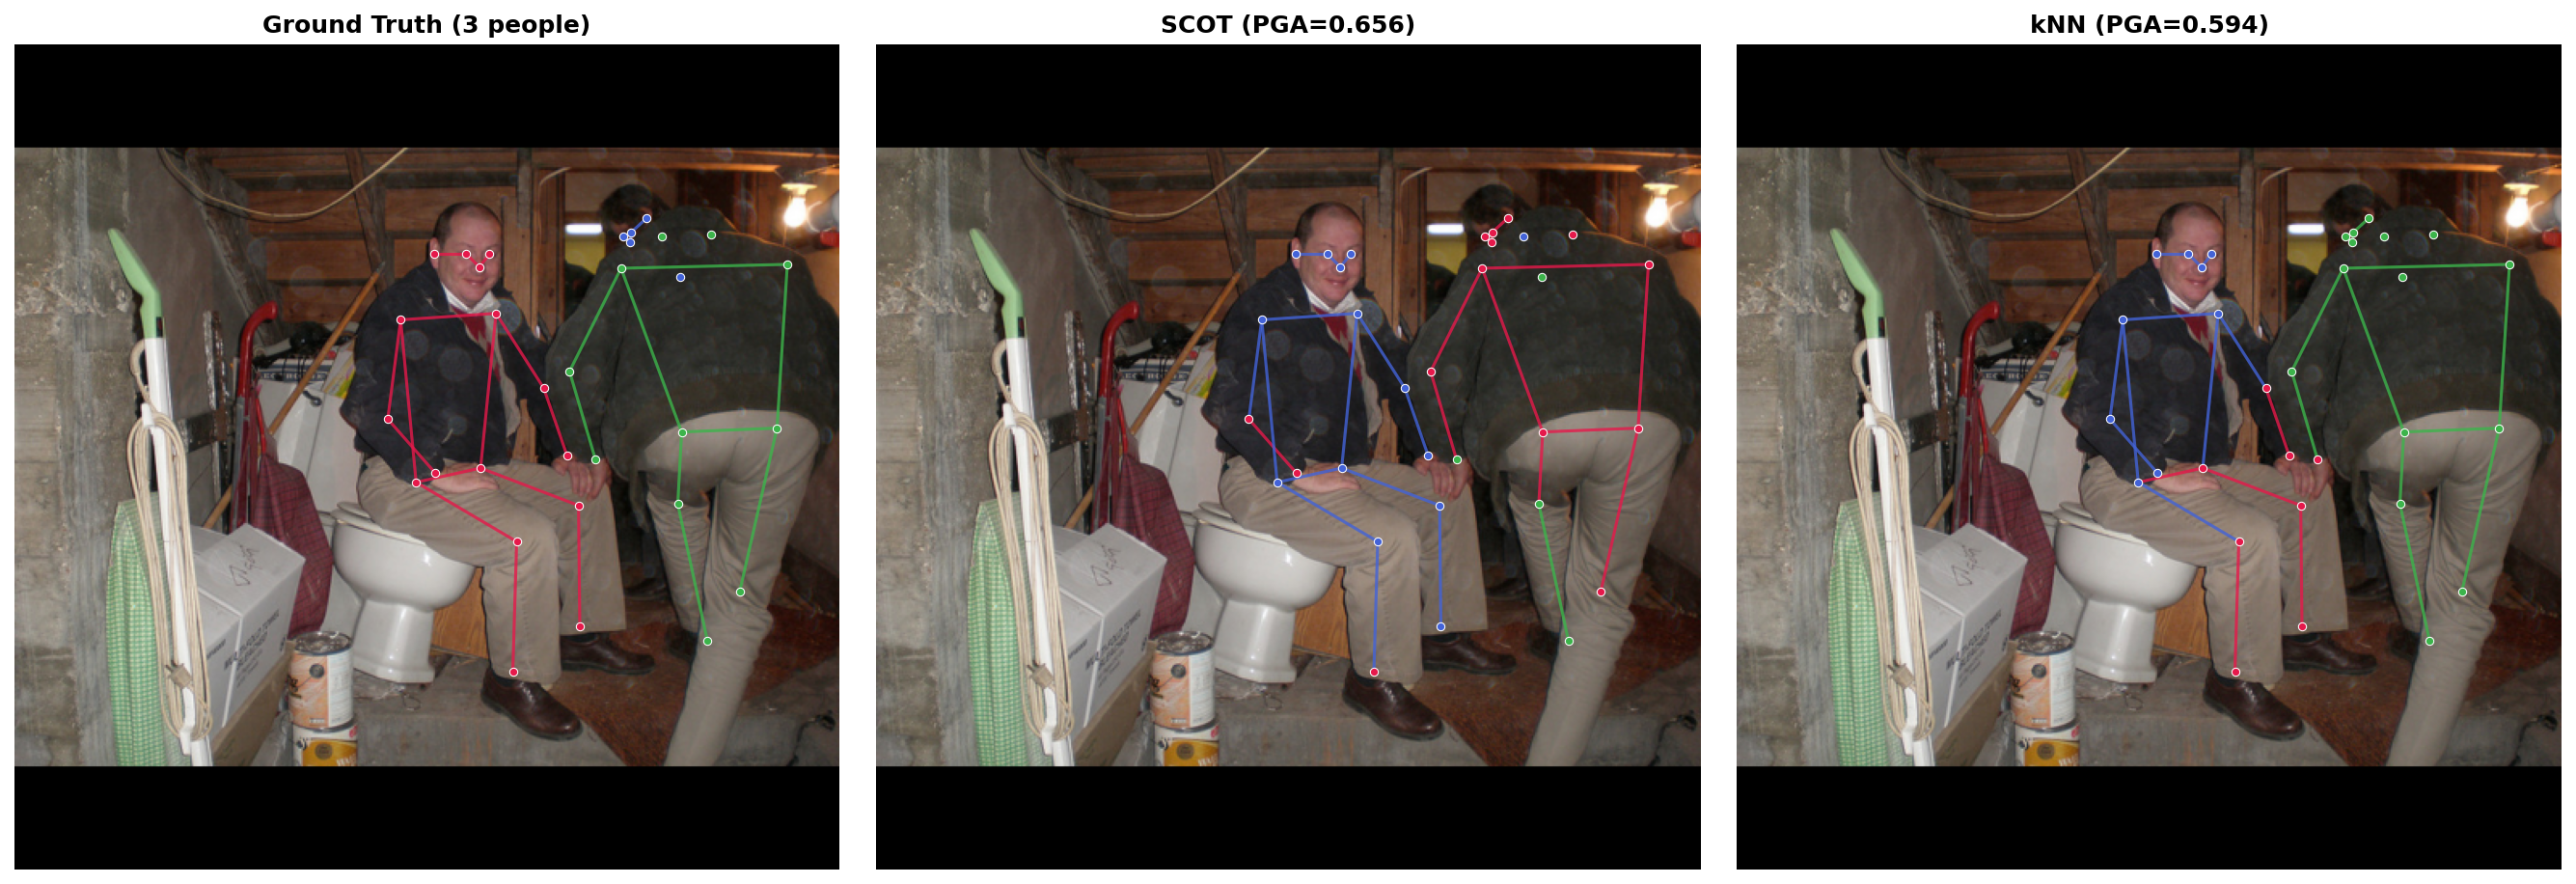
\includegraphics[width=0.9\linewidth]{figures/demo_example_1.png}
    % TODO(figure): replace with a block diagram of PG-GAT showing:
    %   (a) input node features (position, visibility, type embedding)
    %   (b) edge feature constructor producing the 7-dim edge vector
    %       (4-way category one-hot + L2 distance + skeleton hop + same-type flag)
    %   (c) stacked GATv2Conv layers (3 of them per the architecture sweep)
    %       split into a 3-head standard sub-layer and a 1-head repulsion
    %       sub-layer that masks all non-same-type edges
    %   (d) final linear projection + L2 normalisation to embedding dim 256
    % The three colour-highlighted modifications (1: type-pair bias,
    % 2: position encoding, 3: repulsion heads) should be visually
    % distinguishable as the contribution boundaries.
    \caption{The PG-GAT architecture.
    Input node features are the keypoint position, the visibility flag,
    and a learnable joint-type embedding.
    Modification~1 attaches a four-way edge-category one-hot to every edge
    that enters the GATv2 attention as a learned additive bias (red).
    Modification~2 concatenates three geometric edge features
    (L2 distance, skeleton hop distance, same-type indicator)
    onto that one-hot before the same edge encoder (blue).
    Modification~3 splits the multi-head attention into a standard sub-layer
    over the full neighbourhood and a repulsion sub-layer
    whose attention mask restricts it to same-type edges only (green).
    Each modification is independently configurable via a boolean flag,
    which allows the ablation experiments of Chapter~\ref{chap_4} to isolate its marginal contribution.}
    \label{fig:pggat_architecture}
\end{figure}

\subsection{Modification~1: type-pair attention bias}
\label{sec_meth_pggat_typeattn}

Every edge $(i, j) \in \mathcal{E}$ is categorised into one of four mutually exclusive classes based on the joint-type pair $(t_i, t_j)$:
\begin{compactitem}
    \item \textsc{Same-Type} --- $t_i = t_j$, indicating two keypoints that must belong to different people.
        Two left elbows in the same image cannot share an identity.
    \item \textsc{Skeletal-Neighbour} --- $(t_i, t_j)$ is a directly adjacent pair on the COCO skeleton graph (e.g.\ shoulder--elbow).
        The strongest cue for same-person grouping:
        anatomically connected joints from the same person have consistent spatial relationships.
    \item \textsc{Same-Limb} --- $(t_i, t_j)$ lies on the same limb chain but is not directly adjacent (e.g.\ shoulder--wrist).
        Provides medium-range structural information.
    \item \textsc{Cross-Body} --- otherwise.
        Carries weak or no structural prior.
\end{compactitem}
The category is represented as a one-hot vector $\mathbf{c}_{ij} \in \{0,1\}^{4}$
and passed through a small edge-encoder MLP $\phi_{\text{edge}}$ to produce an edge feature
$\mathbf{e}_{ij}^{\text{cat}} = \phi_{\text{edge}}(\mathbf{c}_{ij}) \in \mathbb{R}^{d_e}$.
This edge feature enters the GATv2 attention coefficient via the standard \texttt{edge\_dim} mechanism of PyG's \texttt{GATv2Conv} implementation~\cite{fey2019pyg},
which extends the attention pre-activation by an additive learned edge bias:
\begin{equation}
    \alpha_{ij}^{(l)}
    \propto \exp\!\Bigl(
        \mathbf{a}^{(l)\top}
        \mathrm{LeakyReLU}\!\bigl(
            \mathbf{W}^{(l)} [\,\mathbf{h}_i^{(l)} \,\|\, \mathbf{h}_j^{(l)}\,]
            + \mathbf{W}_e^{(l)} \mathbf{e}_{ij}^{\text{cat}}
        \bigr)
    \Bigr),
    \label{eq:pggat_typeattn}
\end{equation}
where the learnable parameters $\mathbf{a}^{(l)}$, $\mathbf{W}^{(l)}$, and $\mathbf{W}_e^{(l)}$ are GATv2 layer-$l$ weights.
The four edge categories therefore enter the attention as four learnable additive biases that the network can adjust independently
without disturbing the underlying GATv2Conv numerics.

The decision to inject category information as an edge feature rather than as a per-category weight tensor
was made on the basis of an initial implementation that used custom scatter-based attention with per-category projection matrices.
That implementation failed catastrophically (synthetic PGA $0.60$) due to numerical instability in the manual softmax over scattered scores;
switching to GATv2Conv with edge features recovered stable training and removed the instability without affecting expressive power.

\subsection{Modification~2: skeleton-relative position encoding}
\label{sec_meth_pggat_posenc}

The baseline GAT carries no explicit spatial information in its attention coefficients:
positional information is present only as a node feature
and is mixed indiscriminately with the type embedding and visibility.
The second modification injects three geometric edge features
that surface relative-geometry information directly to the attention mechanism:
\begin{compactitem}
    \item the L2 distance between the two endpoints, $\|\mathbf{p}_i - \mathbf{p}_j\|_2$;
    \item the skeleton hop distance $d_{\text{hop}}(t_i, t_j)$, defined as the shortest path between the joint types $t_i$ and $t_j$ on the COCO skeleton graph, normalised to $[0,1]$;
    \item a same-type indicator $\mathbb{1}[t_i = t_j] \in \{0,1\}$.
\end{compactitem}
These three scalars are concatenated with the four-dimensional category one-hot of Modification~1
and the resulting seven-dimensional edge vector
is passed through the same edge-encoder $\phi_{\text{edge}}$ as before.
The skeleton hop distance is the load-bearing component:
it tells the attention layer how anatomically related two keypoint types are,
independently of how spatially close they happen to be in the image.
A shoulder near an elbow (hop $=1$) is expected and the attention can up-weight the message;
a shoulder near an ankle (hop $\geq 3$) is surprising and is likely to be a cross-person collision that should be down-weighted.

\subsection{Modification~3: same-type repulsion heads}
\label{sec_meth_pggat_repulsion}

The third modification dedicates a subset of the multi-head attention to the inter-person discrimination task.
In a standard GAT layer with $H$ heads, every head attends to every neighbour of the centre node;
the gradient signal for distinguishing two same-type keypoints of different people
is therefore averaged across $H$ heads that are simultaneously trying to learn skeletal grouping.
The repulsion modification splits the layer into a standard GATv2Conv that attends to all neighbours
and a smaller repulsion GATv2Conv whose attention mask is restricted to same-type edges only.
The outputs of the two sub-layers are concatenated along the head dimension,
giving the same total head count as the baseline.

Formally, let the standard sub-layer use $H_{\text{std}}$ heads attending to the full neighbourhood $\mathcal{N}(i)$,
and the repulsion sub-layer use $H_{\text{rep}}$ heads attending to the same-type neighbourhood
$\mathcal{N}_{=}(i) = \{j \in \mathcal{N}(i) : t_j = t_i\}$,
with $H_{\text{std}} + H_{\text{rep}} = H$.
The layer-$l$ output is then
\begin{equation}
    \mathbf{h}_i^{(l+1)}
    = \bigl[\, \mathrm{GATv2Conv}_{\text{std}}(\mathbf{h}_i^{(l)}, \mathcal{N}(i))
        \,\big\|\,
        \mathrm{GATv2Conv}_{\text{rep}}(\mathbf{h}_i^{(l)}, \mathcal{N}_{=}(i)) \,\bigr],
    \label{eq:pggat_repulsion}
\end{equation}
where $[\cdot \| \cdot]$ denotes concatenation along the head dimension.
The repulsion sub-layer never sees skeletal-neighbour, same-limb, or cross-body edges,
and the contrastive loss of Equation~\eqref{eq:contrastive_loss} consequently pushes its parameters
to produce discriminative features specifically for the case ``two left elbows --- whose elbows are they?''

The default configuration reserves a single repulsion head out of four ($H_{\text{rep}} = 1$, $H_{\text{std}} = 3$);
this choice was validated by the architecture sweep described in Section~\ref{sec_meth_pggat_training},
which is the same sweep that fixes the depth, hidden dimension, output dimension, and dropout of the PG-GAT layer stack.

\subsection{Composing the modifications and training}
\label{sec_meth_pggat_training}

The three modifications are independently configurable via boolean flags on \texttt{SAGATConfig}\footnote{
The implementation class retains the legacy name \texttt{SAGATConfig};
the method is referred to as PG-GAT throughout this document.}
(\texttt{use\_type\_pair\_attention}, \texttt{use\_position\_encoding}, \texttt{use\_repulsion\_heads}),
which allows each one to be isolated for the ablation experiments reported in Chapter~\ref{chap_4}.
The PG-GAT model used in the headline evaluations enables all three;
the ablation table that reports the marginal contribution of each modification is~Table~\ref{tab:pggat_ablation_headline} in Chapter~\ref{chap_4}.

\paragraph{Architecture defended by Bayesian sweep.}
The architecture hyperparameters (number of layers, number of heads, hidden dimension, output dimension, joint-type embedding dimension, dropout)
are not inherited from the baseline of Section~\ref{sec_meth_baseline}.
Instead, they are selected by a 32-run Bayesian sweep over the six axes,
with the search space chosen to span the smallest values used by prior GNN-on-pose work
up to the memory ceiling at batch size 4 on the experimental hardware.
Selection metric: synthetic validation PGA of Equation~\eqref{eq:pga}.
Hyperband early termination~\cite{li2018hyperband} retires weak configurations at the fifth validation iteration (epoch 25)
to keep the sweep within the overnight budget while preserving late-converging configurations.
The selected configuration --- three layers, four heads, hidden dimension 64, output dimension 256,
joint-type embedding dimension 64, dropout 0.1 ---
is the architecture used by every PG-GAT result in Chapter~\ref{chap_4} and Chapter~\ref{chap_5}.
A complementary loss sweep over the contrastive margin, repulsion head count, learning rate, and weight decay
returned the defaults of Section~\ref{sec_meth_baseline_loss} as near-optimal,
which is itself recorded as evidence that the contrastive bar is already at the right operating point.

\paragraph{Two-stage training.}
Pre-training is conducted on the 400-scene synthetic dataset of Section~\ref{sec_meth_data_synth}
with the optimiser settings of Section~\ref{sec_meth_baseline_training}.
Fine-tuning then proceeds on COCO~\cite{lin2014coco} \texttt{train2017} for a small number of additional epochs at a reduced learning rate;
this second stage adapts the embedding to the COCO image distribution
while retaining the per-person identity structure learned on synthetic data.
The exact fine-tune schedule (epochs, learning rate, weight decay)
is selected by a third Bayesian sweep over a 12-run search space around the legacy inherited recipe of 20 epochs at $10^{-4}$ learning rate.
The selected configuration --- 15 epochs at the sweep-chosen learning rate and weight decay ---
produces the headline numbers reported in Chapter~\ref{chap_4} and is logged under the W\&B alias \texttt{meng-headline}.

\paragraph{Read-out.}
The grouping read-out remains the same $k$-means with $k = K$ on the L2-normalised PG-GAT embeddings
as in the baseline of Section~\ref{sec_meth_baseline_training}.
PG-GAT changes the embedding;
the head stays simple by design.

\subsection{Variants explored after PG-GAT}
\label{sec_meth_pggat_variants}

PG-GAT as described in this section is the defended embedding network
and the source of the headline result reported in Chapter~\ref{chap_4}.
Three independent variants of the PG-GAT design are also reported in Chapter~\ref{chap_4},
each one a controlled stress-test of a different design choice
rather than a competing answer to the grouping problem.
Section~\ref{sec_meth_v2} (PG-GAT v2) tests whether augmenting the positional input with pre-trained visual features extracted by a MobileNetV2 backbone~\cite{sandler2018mobilenetv2} adds identity signal that positions alone cannot provide.
Section~\ref{sec_meth_hyperbolic} (hyperbolic PG-GAT) replaces the Euclidean output space with a Lorentz-model hyperbolic manifold,
on the theoretical motivation that tree-structured data embeds with less distortion in hyperbolic space.
Section~\ref{sec_meth_trigat} (TriGAT) replaces the per-node primitive from a single joint to a skeleton triplet of three connected joints,
on the motivation that the pivot angle of a triplet is a rotation-invariant articulation descriptor that single-joint embeddings do not directly capture.
Chapter~\ref{chap_4} reports all three as negative or marginal results;
their methodologies are recorded here so that the corresponding Chapter~\ref{chap_4} numbers and the Chapter~\ref{chap_5} discussion are interpretable.
